%%%%%%%%%%%%%%%%%%%%%%%%%%%%%%%%%%%%%%%%%
% baposter portrait poster - Single-pixel camera + 3D Gaussian Splatting (Truck scene)
% All numbers come from results/*.csv of the spc-gs repository. Figures are in figs_spc/.
%%%%%%%%%%%%%%%%%%%%%%%%%%%%%%%%%%%%%%%%%
\documentclass[portrait,paperwidth=800mm,paperheight=1000mm,fontscale=0.37]{baposter}
\usepackage{graphicx}
\graphicspath{{figs_spc/}{figures/}}
\usepackage{tabularx}
\usepackage[most]{tcolorbox}
\usepackage{amsmath}
\usepackage{amssymb}
\usepackage{booktabs}
\usepackage{enumitem}
\usepackage{palatino}
\usepackage[font=small,labelfont=bf]{caption}
\usepackage{qrcode}
\usepackage{pgf,tikz}
\usetikzlibrary{arrows.meta,shapes,positioning,calc}

\newcommand{\compresslist}{%
\setlength{\itemsep}{0.5ex}\setlength{\parskip}{0pt}\setlength{\parsep}{0pt}\setlength{\topsep}{0.3ex}}
\definecolor{usmblue}{RGB}{0,62,133}
\definecolor{lightblue}{rgb}{0.145,0.6666,1}
\definecolor{accent}{RGB}{217,95,2}
% Key-number card: big value + label
\newcommand{\card}[3]{%
 \begin{tcolorbox}[enhanced,colback=lightblue!12,colframe=usmblue,boxrule=1.2pt,arc=3mm,%
   left=2mm,right=2mm,top=2mm,bottom=2mm,height=4.4em,valign=center,halign=center]
 {\LARGE\bfseries\color{#3}#1}\par\smallskip{\small #2}%
 \end{tcolorbox}}

\begin{document}

\begin{poster}
{
headerborder=closed,
colspacing=1em,
bgColorOne=white,
bgColorTwo=white,
borderColor=usmblue,
headerColorOne=usmblue,
headerColorTwo=usmblue,
headerFontColor=white,
boxColorOne=white,
textborder=roundedleft,
eyecatcher=true,
headerheight=0.1\textheight,
headershape=roundedright,
headerfont=\Large\bf\textsc,
linewidth=2pt
}
%----------------------------------------------------------------------------------------
{
\includegraphics[height=4.5em]{WACCI_logo.png}}
{\bf\textsc{\Large{How many measurements does a single-pixel camera need?}}\\[0.3ex]
 \textsc{\large From 2D reconstruction to 3D Gaussian Splatting}\vspace{0.1cm}}
{\textsc{
    \large{Francisco Alfaro$^1$ and Ayrton Perez$^2$}\\
    \small{
        $^1$Department of Electronics \quad
        $^2$Department of Informatics\\
        Universidad T\'ecnica Federico Santa Mar\'ia, Chile\\
        \textcolor{blue}{francisco.alfaro@usm.cl, ayrton.perez@usm.cl}
    }
}}
{
\includegraphics[height=6.0em]{usm.png}}

%----------------------------------------------------------------------------------------
\headerbox{Motivation and question}{name=motiv,column=0,row=0}{
\raggedright
A \textbf{single-pixel camera (SPC)} replaces the sensor matrix by one photodetector and a sequence of coded patterns:
a simpler sensor, but \textbf{more measurements per image}. For 3D scenes the cost multiplies, because 3D Gaussian
Splatting (3DGS) needs many views.
\medskip

\begin{tcolorbox}[enhanced,colback=accent!8,colframe=accent,boxrule=1.2pt,arc=2mm,left=2mm,right=2mm,top=1.5mm,bottom=1.5mm]
\textbf{Question.} How much quality is lost in the 2D views, and in the 3D model trained on them, when only
5, 10, 25 or 50\,\% of the measurements are taken? Does the pattern (Hadamard, random, DCT) or the reconstruction
(direct, TV) change the answer?
\end{tcolorbox}
}

%----------------------------------------------------------------------------------------
\headerbox{Measurement model}{name=model,column=0,below=motiv}{
\raggedright
\centering
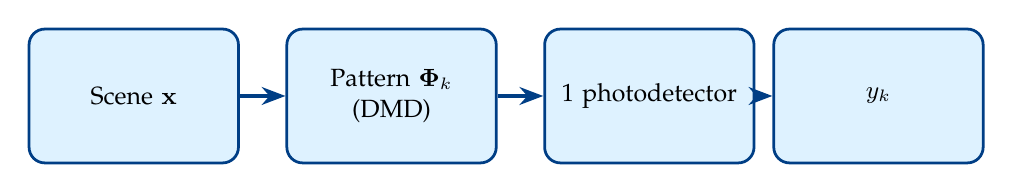
\begin{tikzpicture}[x=\linewidth, nodo/.style={draw=usmblue,fill=lightblue!15,rounded corners=2mm,line width=1pt,minimum height=17mm,
  text width=0.2\linewidth,align=center,font=\small}, flecha/.style={-{Stealth[length=3mm]},line width=1.6pt,usmblue}]
 \node[nodo] (a) at (0.12,0) {Scene $\mathbf{x}$};
 \node[nodo] (b) at (0.39,0) {Pattern $\mathbf{\Phi}_k$ (DMD)};
 \node[nodo] (c) at (0.66,0) {1 photodetector};
 \node[nodo] (d) at (0.9,0) {$y_k$};
 \draw[flecha] (a)--(b); \draw[flecha] (b)--(c); \draw[flecha] (c)--(d);
\end{tikzpicture}
\raggedright\medskip

\[
\mathbf{y}=\mathbf{\Phi}\mathbf{x}+\mathbf{n},\qquad \mathbf{\Phi}\in\mathbb{R}^{K\times N},\quad r=K/N
\]
\noindent One scalar per pattern. Rows of $\mathbf{\Phi}$ are orthonormal ($\mathbf{\Phi}\mathbf{\Phi}^{\top}=\mathbf{I}$) and
are applied with fast transforms, so $\mathbf{\Phi}$ is never stored.
}

%----------------------------------------------------------------------------------------
\headerbox{Patterns and reconstruction}{name=patrones,column=0,below=model}{
\raggedright
\centering
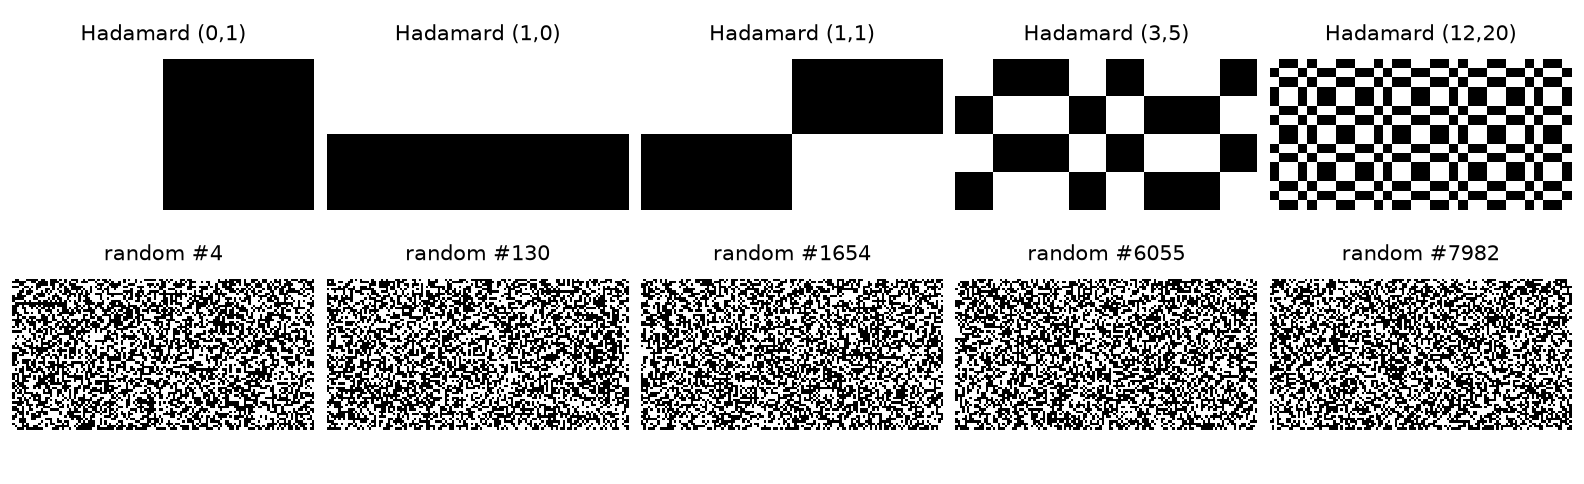
\includegraphics[width=\linewidth]{fig_patterns.png}\\[-0.2ex]
{\small Hadamard (ordered by sequency) and random binary patterns.}
\raggedright\medskip

\begin{itemize}\compresslist
 \item \textbf{Hadamard:} low frequencies first.
 \item \textbf{Random:} permuted Hadamard, DC always measured.
 \item \textbf{DCT:} reference (not binary).
\end{itemize}
\medskip

\noindent\textbf{Direct:} $\hat{\mathbf{x}}=\mathbf{\Phi}^{\top}\mathbf{y}$. \textbf{TV} (FISTA):
\[
\hat{\mathbf{x}}=\arg\min_{\mathbf{x}}\ \tfrac12\|\mathbf{\Phi x}-\mathbf{y}\|_2^2+\lambda\,\mathrm{TV}(\mathbf{x}),\ \ \lambda=0.003
\]
}

%----------------------------------------------------------------------------------------
\headerbox{Cost}{name=costo,column=0,below=patrones}{
\raggedright
\small
\renewcommand{\arraystretch}{1.12}
\begin{tabular*}{\linewidth}{@{}l@{\extracolsep{0pt plus 1fill}}r@{}}
\toprule
Stage & Time \\
\midrule
2D direct & $\le$ 7 ms / view \\
2D TV, 256$\times$512 & 0.99--1.27 s / view \\
2D TV, 512$\times$1024 & 1.69--1.75 s / view \\
3DGS 3000 / 7000 it. & 63--90 s / 146--363 s \\
3DGS 30\,000 it. & 1140--3495 s \\
\bottomrule
\end{tabular*}
\par\smallskip
Peak memory 1.0--4.3\,GiB (SPC).
}

%----------------------------------------------------------------------------------------
\headerbox{Code and references}{name=refs,column=0,below=costo,above=bottom}{
\raggedright
\begin{minipage}[c]{0.36\linewidth}\centering
\qrcode[height=0.95\linewidth]{https://github.com/fralfaro/spc-gs}
\end{minipage}\hfill
\begin{minipage}[c]{0.60\linewidth}\raggedright\small
\textbf{Open source}\\
github.com/fralfaro/spc-gs\\[0.5ex]
Configs, tests and all CSV files.
\end{minipage}

\smallskip
\footnotesize
\noindent [1] Duarte et al., IEEE Signal Process. Mag., 2008.\\
\noindent [2] Yu et al., \textit{cake-cutting}, Sensors, 2019.\\
\noindent [3] Rudin et al., Physica D, 1992.\\
\noindent [4] Beck and Teboulle, SIAM J. Imaging Sci., 2009.\\
\noindent [5] Kerbl et al., ACM TOG, 2023.\\
\noindent [6] Ye et al., gsplat, arXiv:2409.06765, 2024.\\
\noindent [7] Knapitsch et al., ACM TOG, 2017.

\smallskip
\noindent\textit{Claude Code was used as an assistant; the authors checked the results.}
}

%----------------------------------------------------------------------------------------
\headerbox{Experimental pipeline}{name=metodos,column=1,row=0,span=2}{
\centering
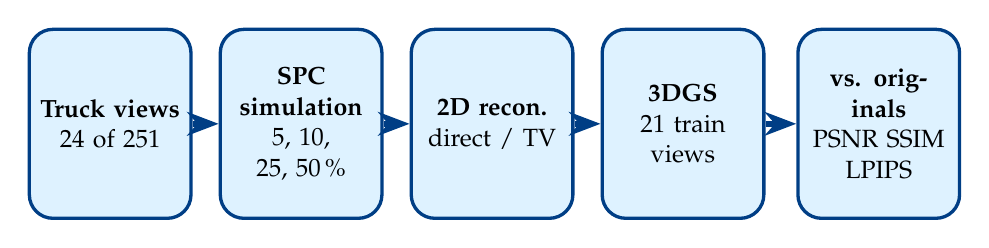
\begin{tikzpicture}[x=\linewidth,
  nodo/.style={draw=usmblue,fill=lightblue!15,rounded corners=3mm,line width=1.2pt,
    minimum width=0.165\linewidth,text width=0.15\linewidth,minimum height=24mm,align=center,font=\small},
  flecha/.style={-{Stealth[length=4mm]},line width=2.2pt,usmblue}]
 \node[nodo] (a) at (0.085,0)  {\textbf{Truck views}\\24 of 251};
 \node[nodo] (b) at (0.285,0) {\textbf{SPC simulation}\\5, 10, 25, 50\,\%};
 \node[nodo] (c) at (0.485,0)  {\textbf{2D recon.}\\direct / TV};
 \node[nodo] (d) at (0.685,0) {\textbf{3DGS}\\21 train views};
 \node[nodo] (e) at (0.89,0)  {\textbf{vs. originals}\\PSNR SSIM LPIPS};
 \draw[flecha] (a.east)--(b.west); \draw[flecha] (b.east)--(c.west);
 \draw[flecha] (c.east)--(d.west); \draw[flecha] (d.east)--(e.west);
\end{tikzpicture}

\medskip
\raggedright
\begin{minipage}[t]{0.56\linewidth}\vspace{0pt}\raggedright
\begin{itemize}\compresslist
 \item \textbf{Scene:} Truck (Tanks and Temples), 979$\times$546; 3 test views, 21 training views, 230 held-out views.
 \item \textbf{Grids:} 256$\times$512 (25\,\% of the pixels) and 512$\times$1024 (98\,\%).
 \item \textbf{Control:} resample to the grid and back, no SPC. \textbf{Baseline:} 3DGS on original images.
 \item \textbf{Metrics} always against the \emph{original} images, full resolution.
\end{itemize}
\end{minipage}\hfill
\begin{minipage}[t]{0.40\linewidth}\vspace{0pt}\raggedright
\begin{tcolorbox}[enhanced,colback=lightblue!10,colframe=usmblue,boxrule=1pt,arc=2mm,left=2mm,right=2mm,top=1mm,bottom=1mm,
  title={\small\bfseries Hardware and software},fonttitle=\small\bfseries,coltitle=white,colbacktitle=usmblue]
 \small RTX 4060 Laptop (8\,GB), WSL2 Ubuntu 24.04, CUDA 12.8, gsplat 1.5.3. Seed 449. Noise off in the main results.
\end{tcolorbox}
\end{minipage}
}

%----------------------------------------------------------------------------------------
\headerbox{2D results}{name=res2d,column=1,span=2,below=metodos}{
\raggedright
\begin{minipage}[t]{0.40\linewidth}\vspace{0pt}\raggedright
\textbf{PSNR (dB)}, grid 256$\times$512, 24 views
\smallskip

\small
\renewcommand{\arraystretch}{1.15}
\begin{tabular*}{\linewidth}{@{}l@{\extracolsep{0pt plus 1fill}}cccc@{}}
\toprule
Pattern, method & 5\,\% & 10\,\% & 25\,\% & 50\,\% \\
\midrule
Hadamard, direct  & 20.63 & 21.89 & 23.92 & 25.92 \\
Hadamard, TV      & 21.52 & 22.89 & 24.87 & 26.33 \\
Random, direct & 12.65 & 12.93 & 13.87 & 15.82 \\
Random, TV      & 20.35 & 21.89 & 24.39 & 26.12 \\
DCT, TV      & \textbf{21.80} & \textbf{23.18} & \textbf{25.17} & \textbf{26.49} \\
\midrule
Control (no SPC) & \multicolumn{4}{c}{27.22} \\
\bottomrule
\end{tabular*}
\normalsize
\smallskip

\small
\begin{itemize}\compresslist
 \item Loss vs. control with Hadamard + TV: \textbf{5.70, 4.33, 2.35, 0.89\,dB}.
 \item TV adds 0.4 to 1.0\,dB over direct.
 \item Random needs TV: direct fails (12.7 to 15.8\,dB).
\end{itemize}
\end{minipage}\hfill
\begin{minipage}[t]{0.58\linewidth}\vspace{0pt}
\centering
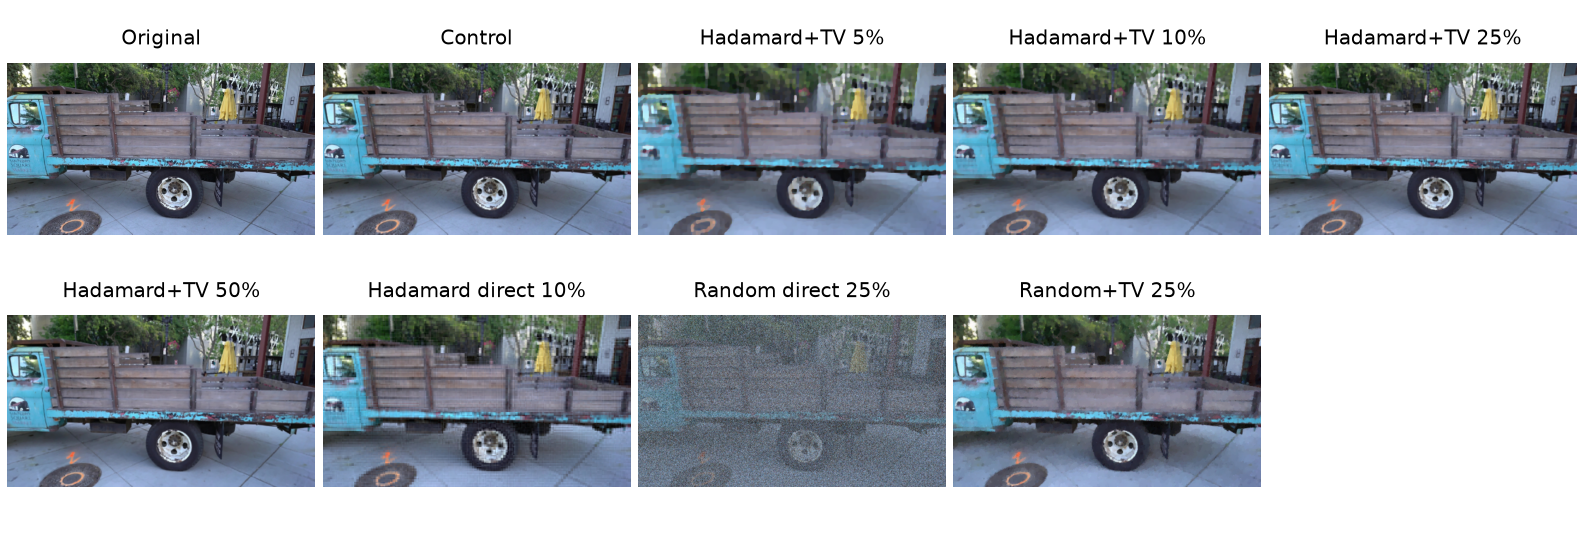
\includegraphics[width=\linewidth]{fig_2d_visual.png}\\[0.2ex]
{\small Training view 000208. TV recovers the slats and wheel from 25\,\%.}
\medskip

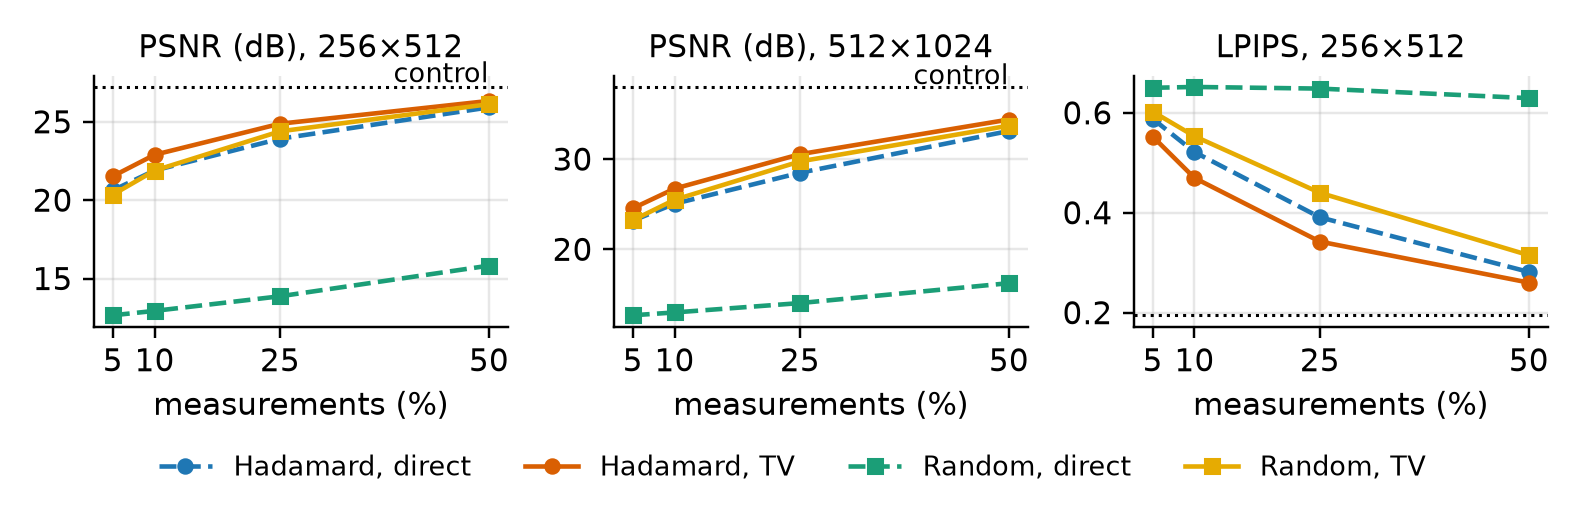
\includegraphics[width=\linewidth]{fig_2d_metrics.png}\\[0.2ex]
{\small Quality vs. measurement ratio on both grids.}
\end{minipage}
}

%----------------------------------------------------------------------------------------
\headerbox{3D results (3DGS, 7000 iterations)}{name=res3d,column=1,span=2,below=res2d}{
\raggedright
\begin{minipage}[t]{0.315\linewidth}\vspace{0pt}\card{19.38 dB}{Held-out PSNR, Hadamard + TV 50\,\% (baseline 19.40)}{usmblue}\end{minipage}\hfill
\begin{minipage}[t]{0.315\linewidth}\vspace{0pt}\card{$\approx$ 2D}{Training views inherit the 2D loss (25.90 vs. 26.33 dB at 50\,\%)}{accent}\end{minipage}\hfill
\begin{minipage}[t]{0.315\linewidth}\vspace{0pt}\card{3 views}{test PSNR is not conclusive: 17 of 42 pairs}{usmblue}\end{minipage}

\medskip
\begin{minipage}[t]{0.60\linewidth}\vspace{0pt}\centering
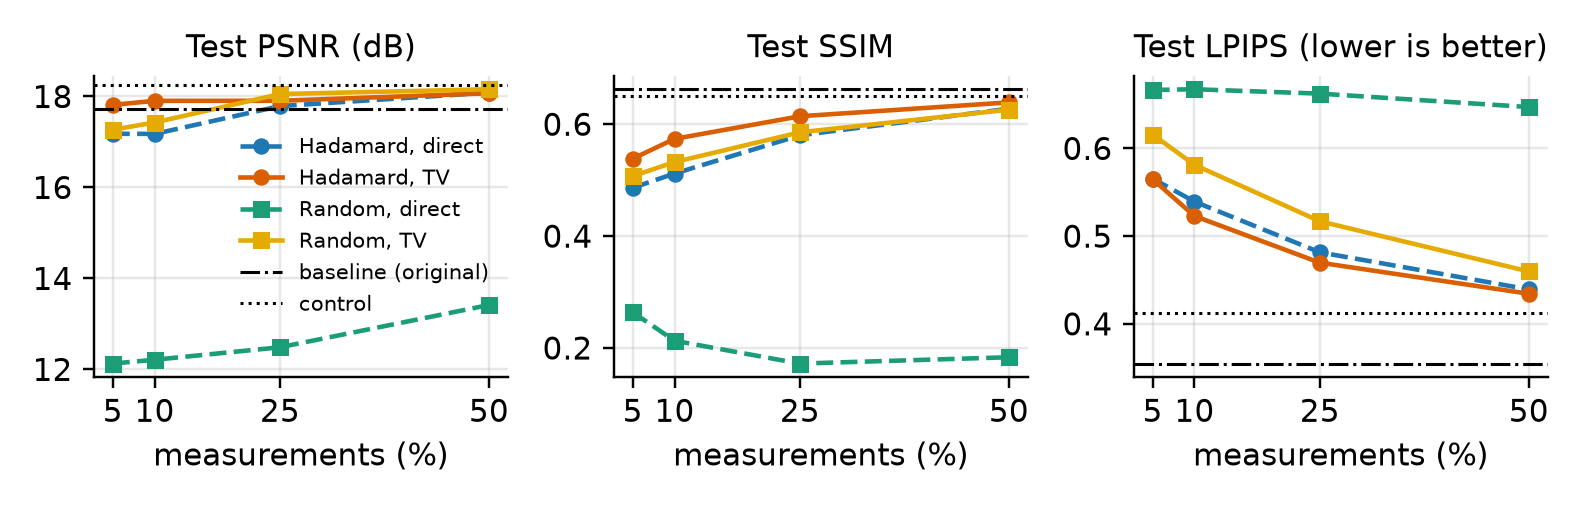
\includegraphics[width=\linewidth]{fig_3d_test.png}\\[0.2ex]
{\small Three test views: PSNR is flat, SSIM and LPIPS order the conditions.}
\end{minipage}\hfill
\begin{minipage}[t]{0.37\linewidth}\vspace{0pt}\centering
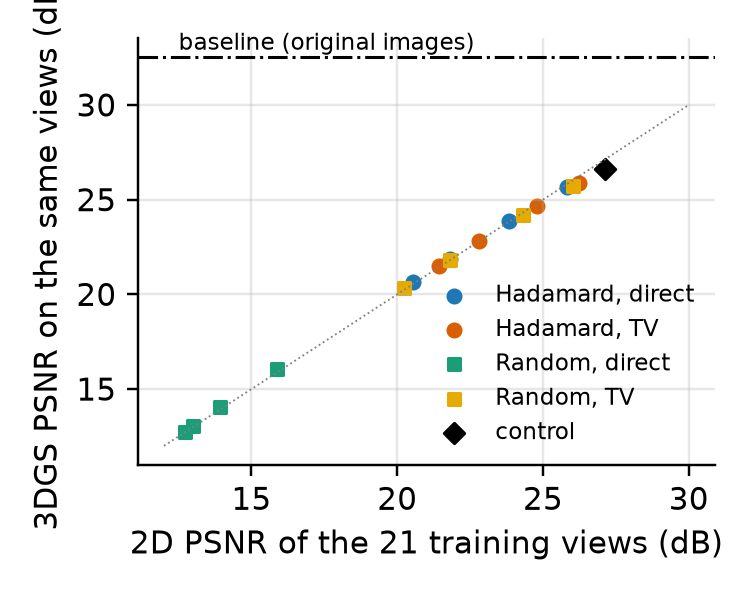
\includegraphics[width=\linewidth]{fig_2d_to_3d.png}\\[0.2ex]
{\small 2D vs. 3D PSNR on training views.}
\end{minipage}

\medskip
\centering
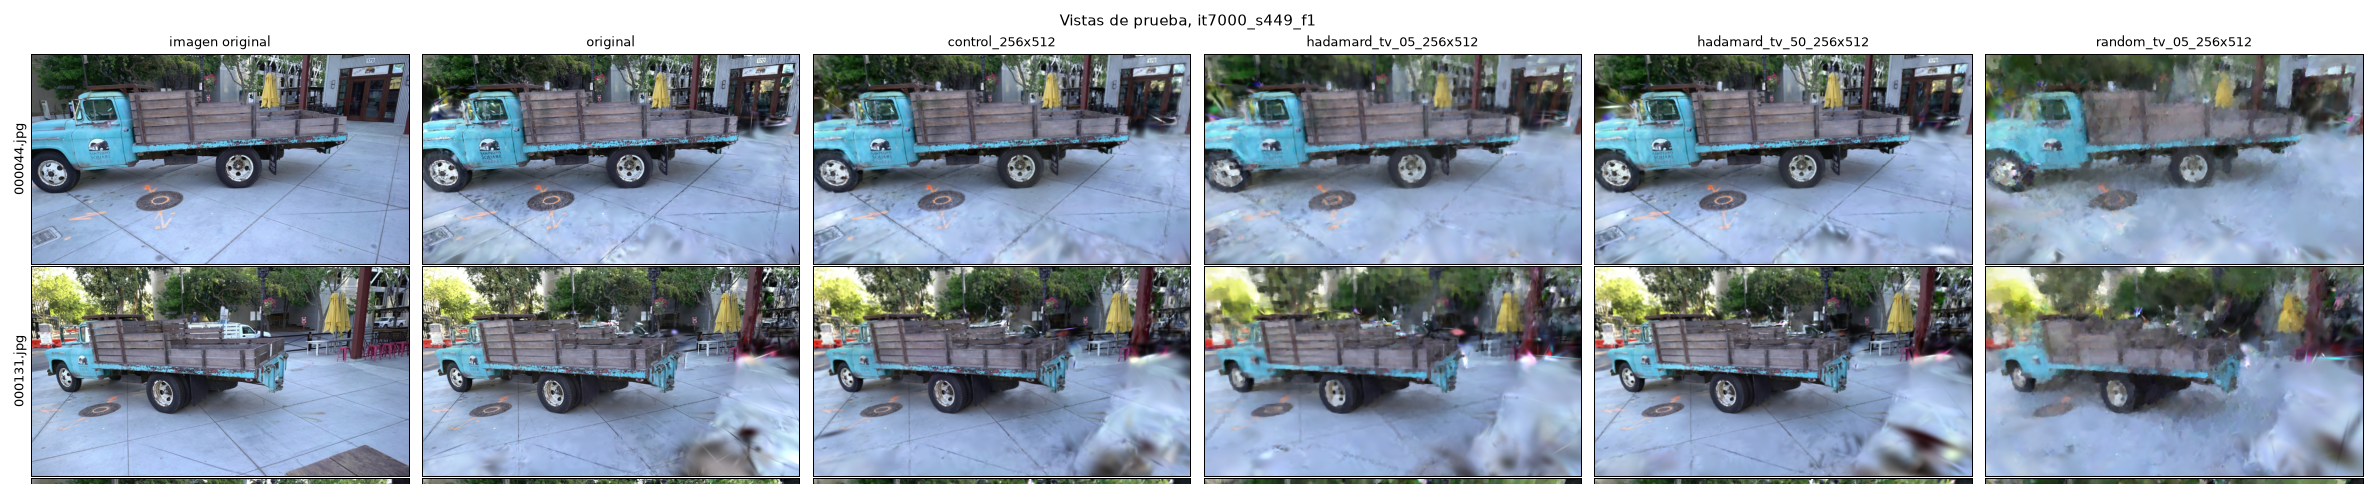
\includegraphics[width=0.78\linewidth]{fig_3d_renders.png}\\[-0.2ex]
{\small Test views 000044 and 000131 (columns: original image, baseline, control, Hadamard + TV 5\,\% and 50\,\%, random + TV 5\,\%).}
}

%----------------------------------------------------------------------------------------
\headerbox{Conclusions and limits}{name=concl,column=1,span=2,below=res3d,above=bottom}{
\raggedright
\begin{itemize}\compresslist
 \item \textbf{2D:} Hadamard + TV loses 0.89\,dB at 50\,\% and 5.70\,dB at 5\,\% vs. the control.
 \item \textbf{3D:} 3DGS inherits the 2D loss; with 230 held-out views, 50\,\% matches the baseline.
 \item \textbf{Limits:} one scene, one seed, COLMAP poses from original images (optimistic), simulated optics.
 \item \textbf{Next:} more scenes, re-estimated poses, 3DGS from the measurements.
\end{itemize}
}

\end{poster}

\end{document}
